\section{Real Data Applications}
\label{Sec:DA}

We  now present an application of our proposed approach to some real data problems. 

Robust techniques are useful when in identifying outlying observations, and we illustrate 
below how to make use of our fixed-dimensional methods presented earlier for 
functional (and hence infinite-dimensional)  data. 

We follow the approach of \cite{ref:JASA151100_BoenteSalibianBarrera} 
for performing robust principal component 
analysis on functional data using the estimated eigenvectors from 
$\widehat{\tilde{\Sigma}}$. Suppose the data consistents of  $n$ curves, say 
$ \cF = \{ f_1, \ldots , f_n  \} \in L^2[0,1]$, each observed at a set of common design 
points $\{ t_1, ..., t_m \} $. We model each of these functions as a linear combination of 
$p$ mutually orthogonal B-spline basis functions $\cD = \{ \delta_1, ..., \delta_p \}$. We map data for each of the functions onto the coordinate system formed by the spline basis:
%
\begin{equation}
T( \cF, \cD)_{ij} = \sum_{l=2}^m f_i(t_l) \delta_j(t_l) (t_l - t_{l-1}); \quad 1 \leq i \leq n, 1 \leq j \leq p.
\end{equation}
%
We then model  the $i$-th row of the $n \times p$ matrix $T(\cF, \cD) \equiv T$, 
denoted by $\bfT_{i}$ 
as follows:
\ban 
\bfT_i = \mu + P s_i + e_{i},
\ean
where $\mu$ is a location parameter, $P$ is a $p \times q$ loading matrix, $s_{i}$ is 
a $q \times 1$ score vector, and $e_{i}$ is the error term. We obtain robust estimators of 
$\mu$, $P$ and consequently $s_{i}$ using $\widehat{\tilde{\Sigma}}$. Define 
$\widehat{\bfT}_{i} = \hat{\mu} + \hat{P} \hat{s}_{i}$. 
The \textit{orthogonal distance} (OD)  corresponding to this projection is defined as 
\ban 
OD_{i} = | \bfT_i - \widehat{\bfT}_{i} |.
\ean
Analogously, the \textit{score distance} (SD) is defined as 
\ban 
SD_i = \sqrt{ \sum_{j=1}^q \frac{\hat{s}^2_{ij}}{\hat \lambda_j}}; 
\ean
where $\hat \lambda_1,\ldots ,\hat \lambda_q$ are the top eigenvalues from 
$\widehat{\tilde{\Sigma}}$. 
%We also transform this approximation back to the original coordinates: 
%$\hat f_i (t_l) = \sum_{j=1}^p \widehat{\bfT}_{ij} \delta_j (t_l)$. 
For outlier detection, following \cite{ref:Technometrics0564_Hubertetal} 
we set the upper cutoff values for 
score distances at $(\chi^2_{2, .975})^{1/2}$ and orthogonal distances at 
\ban
[\text{median}(OD^{2/3}) + \text{MAD}(OD^{2/3})\Phi^{-1}(0.975)]^{3/2},
\ean
 where 
$\Phi(\cdot)$ is the standard normal cumulative distribution function.

\begin{figure}[t!]
\begin{center}
\begin{tabular}{ll}
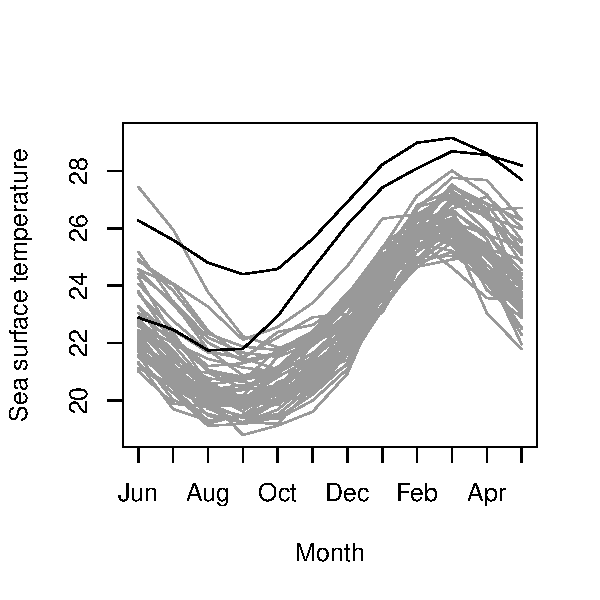
\includegraphics[width=0.4\textwidth]{./Plots/Elnino_functional1} &
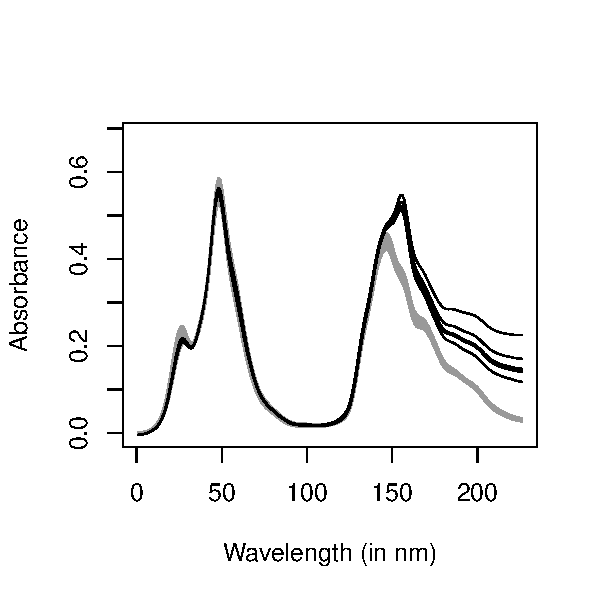
\includegraphics[width=0.4\textwidth]{./Plots/Octane_functional1}\\
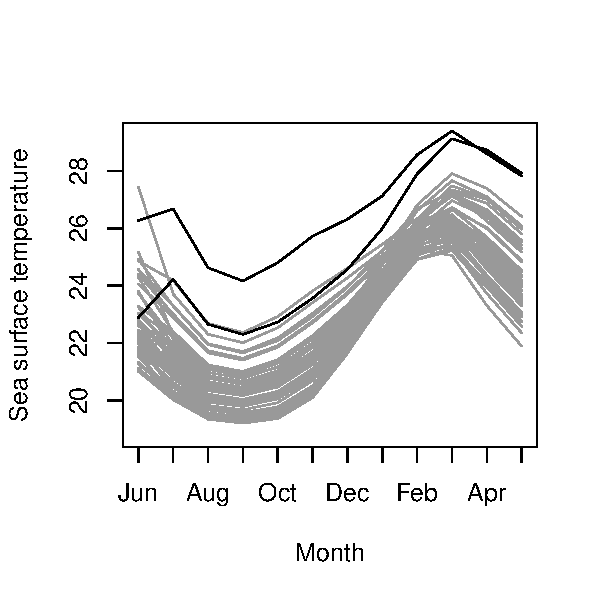
\includegraphics[width=0.4\textwidth]{./Plots/Elnino_functional2} &
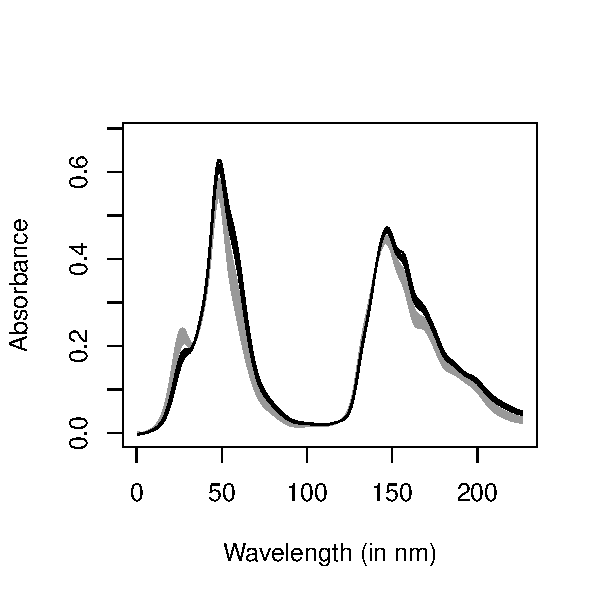
\includegraphics[width=0.4\textwidth]{./Plots/Octane_functional2}\\
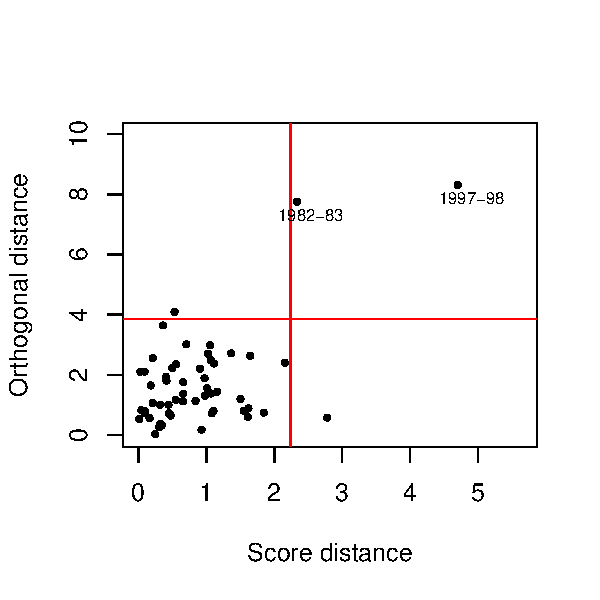
\includegraphics[width=0.4\textwidth]{./Plots/Elnino_functional3} &
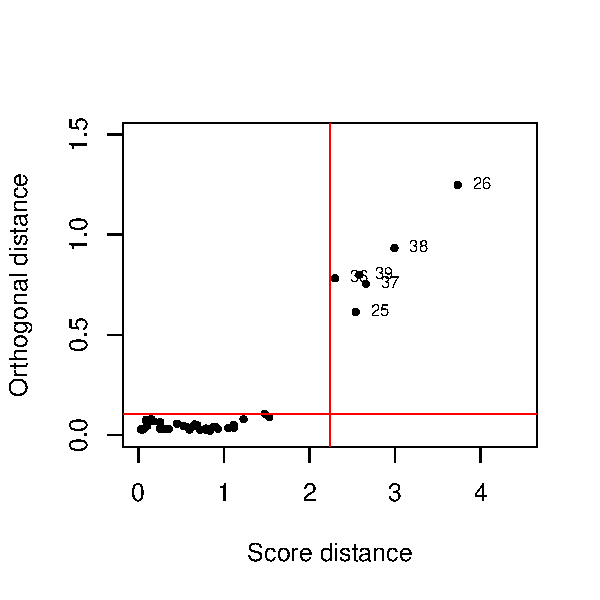
\includegraphics[width=0.4\textwidth]{./Plots/Octane_functional3}\\
\end{tabular}
\caption{Actual sample curves, their spline approximations and diagnostic plots respectively for El-Ni\~no (a,c,e) and Octane (b,d,f) datasets}
\label{fig:fPCAfig}
\end{center}
\end{figure}

We apply the above outlier detection method on two data sets. First, we consider the 
monthly average \textit{sea surface temperature anomaly data} 
from June 1970 to May 2004, available 
from \url{http://www.cpc.ncep.noaa.gov/data}, depicted in  panel (a) 
of Figure~\ref{fig:fPCAfig})).
Second, we consider the \textit{octane data}, which consists of 226 variables and 39 
observations \citep{ref:EsbensenetalBook94}. 
Each sample is a gasoline compound with a certain octane 
number, and has its NIR absorbance spectra measured in 2 nm intervals between 1100 - 1550 
nm. There are 6 outliers here: compounds 25, 26 and 36-39, which contain alcohol. This 
data is presented in  panel (b) of Figure~\ref{fig:fPCAfig})).

In the sea surface temperature data, using a cubic spline basis with knots at alternate 
months starting in June, we get a close approximation as depicted in 
panel (c) of Figure~\ref{fig:fPCAfig}. Using our proposed methodology with $q =1$ 
results in two points having their SD and OD larger than cutoff, depicted in  
panel (e) of Figure~\ref{fig:fPCAfig}. These points correspond to the time periods June 
1982 to May 1983 and June 1997 to May 1998 are marked by black curves in panels a and c, 
and pinpoint the two seasons with strongest El-Ni\~no events. 


On the octane data, we use the same methodology, 
 and again the top robust PC turns out to be sufficient in identifying all 6 outliers. 
 Details are available in  panels (b), (d) and (f) of Figure~\ref{fig:fPCAfig}.